\subsection{Handicaps}

Les Handicaps\footnotemark[1] représentent les défauts qui compliquent parfois la vie de votre personnage. Certains sont plus contraignant que d'autres et certains dépendent du scénario. Ils permettent de choisir des Atouts supplémentaires mais surtout ajoute du caractère à votre personnage et augmente ainsi sont intérêt et votre plaisir de jouer.

\footnotetext[1]{Comme pour les compétences, je rentre pas dans le détail, hors mis pour les Handicaps qui changent par rapport à l'original de Savage World.}

\begin{description}[align=left]
    \item [Âgé (Majeur)]
        Votre héros se fait vieux, certes, mais n’est pas encore prêt pour l’hospice.
    \item [Anémique (Mineur)]
        Votre héros est particulièrement sensible aux maladies, à la fatigue et aux effets de l’environnement.
    \item [Arrogant (Majeur)]
        Votre héros ne pense pas qu’il est le meilleur, il sait qu’il l’est.
    \item [Aveugle (Majeur)]
        Votre héros complètement aveugle, il ne voit rien du tout.
    \item [Bavard (Mineur)]
        On dit qu’une grande gueule peut couler un navire. Votre héros l’est au point qu’il pourrait couler une armada.
    \item [Bizarrerie (Mineur)]
        Votre héros possède une bizarrerie, rien de grave, mais pouvant lui causer des ennuis. Genre ne pas se battre avant d'être présenter, frapper trois fois à la porte avant de pouvoir entrer\ldots
    \item [Boiteux (Majeur)]
        Une vieille blessure a presque estropié votre héros.
    \item [Borgne (Majeur)]
        Votre héros a dans le passé eu l’\oe{il} crevé par un ennemi.
    \item [Chimères (Mineur ou Majeur)]
        Votre héros croit en des choses qui paraissent étranges pour les autres.
    \item [Couard (Majeur)]
        Tout le monde n’a pas des nerfs d’acier. Votre héros blêmit à la vue du sang et est terrifié à l’idée même de subir une blessure.
    \item [Code d’Honneur (Majeur)]
        L’honneur est très important aux yeux de votre personnage.
    \item [Cupide (Mineur ou Majeur)]
        Votre héros est un grippe-sou qui mesure sa valeur en crédits.
    \item [Curieux (Majeur)]
        C’est un vilain défaut et votre personnage est très vilain.
    \item [Deux mains gauches (Mineur)]
        Certaines personnes ne sont tout simplement pas douées avec la technologie.
    \item [Dur d’Oreille (Mineur ou Majeur)]
        Un personnage ayant perdu tout ou partie de son acuité audition possède ce handicap.
    \item [Ennemi (Mineur ou Majeur)]
        Quelqu’un quelque part déteste votre héros et veut sa mort.
    \item [Étranger (Mineur)]
        Votre héros n’appartient pas à la société dans laquelle il vit.
    \item [Frêle (Majeur)]
        Votre héros est, soit très petit, soit très maigre, voire les deux par rapport à la norme de son peuple.
    \item [Gamin (Majeur)]
        Il arrive que des événements incroyables poussent des enfants vers l’aventure. Sachez que choisir ce Handicap signifie débuter avec un gros désavantage.    
    \item [Héroïque (Majeur)]
        Votre héros ne dit jamais non à une personne dans le besoin. Cela peut ne pas lui plaire mais il se sent obligé de secourir ceux qu’il considère sans défense.    
    \item [Ignorant (Majeur)]
        Votre héros en sait moins que les autres sur le monde dans lequel il vit.
    \item [Illettré (Mineur)]
        Votre héros ne sait pas lire.
    \item [Loyal (Mineur)]
        Votre personnage n’est peut-être pas l’archétype du héros, mais il donnerait sa vie pour ses amis.
    \item [Malchanceux (Majeur)]
        Votre héros est moins chanceux que les autres.
    \item [Manchot (Majeur)]
        Votre héros est né avec un seul bras ou l’a perdu lors d’un combat passé.
    \item [Mauvaise habitude (Mineur ou Majeur)]
        Votre héros possède une manie grossière et porte sur les nerfs de son entourage.
    \item [Moche (Mineur)]
        La nature n’a pas été tendre concernant l’apparence de votre héros.
    \item [Myope (Mineur ou Majeur)]
        La vue de votre héros n’est plus ce qu’elle était.
    \item [Obèse (Mineur)]
        Les personnes corpulentes éprouvent rapidement de grandes difficultés lors des situations physiques dangereuses.
    \item [Pacifiste (Mineur ou Majeur)]
        Votre héros déteste la violence et ne se bat jamais ou en d'exceptionnelles circonstences.
    \item [Phobie (Mineur ou Majeur)]
        Les phobies sont des peurs irrationnelles qui empoisonnent le héros pour le reste de sa vie.
    \item [Poches percées (Mineur)]
        Le dicton dit qu’un idiot et son argent ne font pas bon ménage. Votre héros est l’idiot en question.
    \item [Prudent (Mineur)]
        Ce personnage incarne l’extrême prudence. Il ne prend aucune décision hâtive.
    \item [Présomptueux (Majeur)]
        Rien ne peut résister à votre héros. C’est du moins ce qu’il croit.
    \item [Rancunier (Mineur ou Majeur)]
        Votre héros n’oublie jamais les offenses qui lui sont faites. La vengence est un plat qui se mange froid.
    \item [Recherché (Mineur ou Majeur)]
        Votre héros a commis un crime dans son passé et sera arrêté s’il est repris par les autorités.
    \item [Rien à perdre (Mineur)]
        N’avoir Rien à perdre ne signifie pas que votre héros est suicidaire mais qu’il ne tient à la vie que pour atteindre un but qu’il s’est fixé.
    \item [Sale caractère (Mineur)]
        Votre héros est désagréable et a très mauvais caractère.
    \item [Sanguinaire (Majeur)]
        Votre héros ne fait jamais de prisonniers à moins d’être sous la surveillance étroite d’un supérieur.
    \item [Sceptique (Mineur)]
        Les sceptiques ne croient au surnaturel que quand ils sont à moitié avalés par une créature surnaturelle.
    \item [Serment (Jedi ou Sith) (Majeur)]
        Le personnage a prêté serment il ne peut s'y soustraire.
    \item [Têtu (Mineur)]
        Votre héros veut toujours avoir raison et n’admettra jamais ses torts.
    \item [Unijambiste (Majeur)]
        Avec une béquille (ou une jambe de bois).
\end{description}

\begin{paperbox}{Serment (Jedi / Sith)}
    Cet handicap n'est accessible que pour personnages disposant de l'attribut \^Ame à d12 au moins et l'attribut Arcane (Force) enfin le personnage doit être au minimum Vétéran. 

    En effet cet handicap représente l'appartenant à un ordre, Jedi ou Sith et donne accès aux Atouts Padawan/Apprenti et Maître Jedi/Seigneur Sith. Avant de pouvoir préter serment, un héro doit maitriser la force et suivre une formation c'est pourquoi il ne peur accéder à cet Handicap en tant que Novice ou Aguerri.

    Cet handicap oblige le joueur à suivre le code de son ordre à la letter sous peine de succomber à la Force et de devenir incontrolable (PNJ).

    Voir le chapitre sur La Force~\ref{sec:force} (p. \pageref{sec:force}) pour plus de détails.
\end{paperbox}

\newpage
\vspace*{\fill}
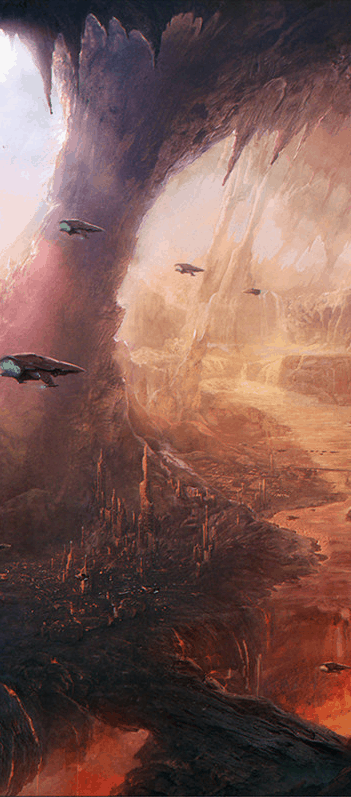
\includegraphics[width=\linewidth]{img/personnages/handicap.png}
